%!TEX encoding = UTF-8 Unicode
%!TEX program = xelatex

\documentclass[bachelor]{swjtuthesis}
% bachelor|master|doctor [professional] [english] [pdf] [authoryear|numebers]
\usepackage{swjtuextra}
\usepackage{enumitem}
\usepackage{subfigure}
\usepackage{wrapfig}
\graphicspath{{figures/}}

\title{西南交通大学\\基于异构处理器的图像识别系统}
\grade{2015级}
\classifiedindex{国内图书分类号: XXX}
\UDC{国际图书分类号: XXX}
\author{孙齐伟}
\major{电子科学与技术(微电子技术)}
\supervisor{邸志雄}
\secrettext{密级: 公开}
% \cosupervisor{\ 教授}
% \date{二〇一八年三月十五日}    % 注释掉则为今日
% \professionaltype{专业学位类型}
% \secrettext{机密\quad 小于等于20年}    % 内部|秘密|机密,注释本行则不保密

\entitle{Image recognition system based on heterogeneous processor}
\engrade{2015}
\enclassifiedindex{ClassifiedIndex: XXX}
\enUDC{U.D.C: XXX}
\enauthor{Qiwei Sun}
\enmajor{Electronic Science and Technology (Microelectronics)}
\ensupervisor{Zhixiong Di}
% \encosupervisor{Prof. }
% \endate{March 15, 2018}    % today if commented
% \enprofessionaltype{Professional degree type}
% \ensecrettext{Confidential\quad Less than or equal to 20 years}
% Internal|Secret|Confidential

\begin{document}

\maketitle

% 本科论文:
%   frontmatter: 致谢、目录、中文摘要、英文摘要
%   mainmatter: 正文章节、参考文献
%   appendix: 附录
%
% 硕博论文:
%   frontmatter: 中文摘要、英文摘要、目录、符号说明
%   mainmatter: 正文、参考文献
%   appendix: 附录
%   backmatter: 致谢、发表论文

\frontmatter
%!TEX root =  ../main.tex

\begin{abstract}
  摘要是论文内容的总结概括,应简要说明论文的研究目的、基本研究内容、 研究方法或
  过程、结果和结论,突出论文的创新之处。摘要中不宜使用公式、图表,不引用文献。
  博士论文中文摘要一般800~1000个汉字,硕士论文中文摘要一般600个汉字。英文摘要的
  篇幅参照中文摘要。

  关键词另起一行并隔写在摘要下方,一般3~8个词,中文关键词间空一字或用分号“;”隔
  开。英文摘要的关键词与中文摘要的关键词应完全一致,中间用逗号“,”或分号“;”隔开。

  \keywords{西南交通大学;学位论文;\LaTeX{} 模板;学士;硕士;博士}
\end{abstract}

\begin{enabstract}
  This is a sample document of SWJTU thesis \LaTeX{} template for bachelor,
  master and doctor. The template is created by geosciman from zepinglee, which
  orignate from the template created by ywg. The template meets the
  equirements of SWJTU theiss writing standards.

  This document will show the usage of basic commands provided by \LaTeX{} and
  some features provided by the template. For more information, please refer to
  the template document swjtuthesis.pdf.

  \enkeywords{Southwest Jiaotong University (SWJTU); Thesis;
  \LaTeX{} Template; Bachelor; Master; PhD}
\end{enabstract}

\tableofcontents
\listoffigures
\listoftables
% \listofalgorithms
% \input{chapters/0.notation}


\mainmatter
\chapter{绪论}

\section{研究背景与意义}
    随着微电子技术的发展,硬件计算水平已经达到了前所未有的高度,这促使九十年代一度被人忽视的神经网络算法得到飞速发展,尤其是在图像识别领域,神经网络越来越受到人们的重视。
    神经网络具有自适应学习能力,也可以根据不同的需求更改网络的复杂度,同时对噪声不太敏感,相比与传统的识别方法,神经网络算法具备更高的鲁棒性。

    时下,由于神经网络算法中存在这海量的参数、复杂的计算过程,因此传统的方法是通过CPU + GPU/TPU架构进行模型的训练工作,这种方法利用了GPU多核、并行计算的特性取得了十分显著的效果。
    但这种架构需要数百瓦的功率支持,同时需要较大的物理空间放置设备,缺乏灵活性,无法满足IoT领域的要求。

    针对IoT领域对续航、灵活性的需求,异构计算芯片成为了极佳的解决方案。当前,一些基于异构处理器的边缘计算方案已经取得了令人瞩目的成绩,例如Google近期推出的搭载了TPU的单板计算机——Coral。
    \begin{figure}
        \centering
        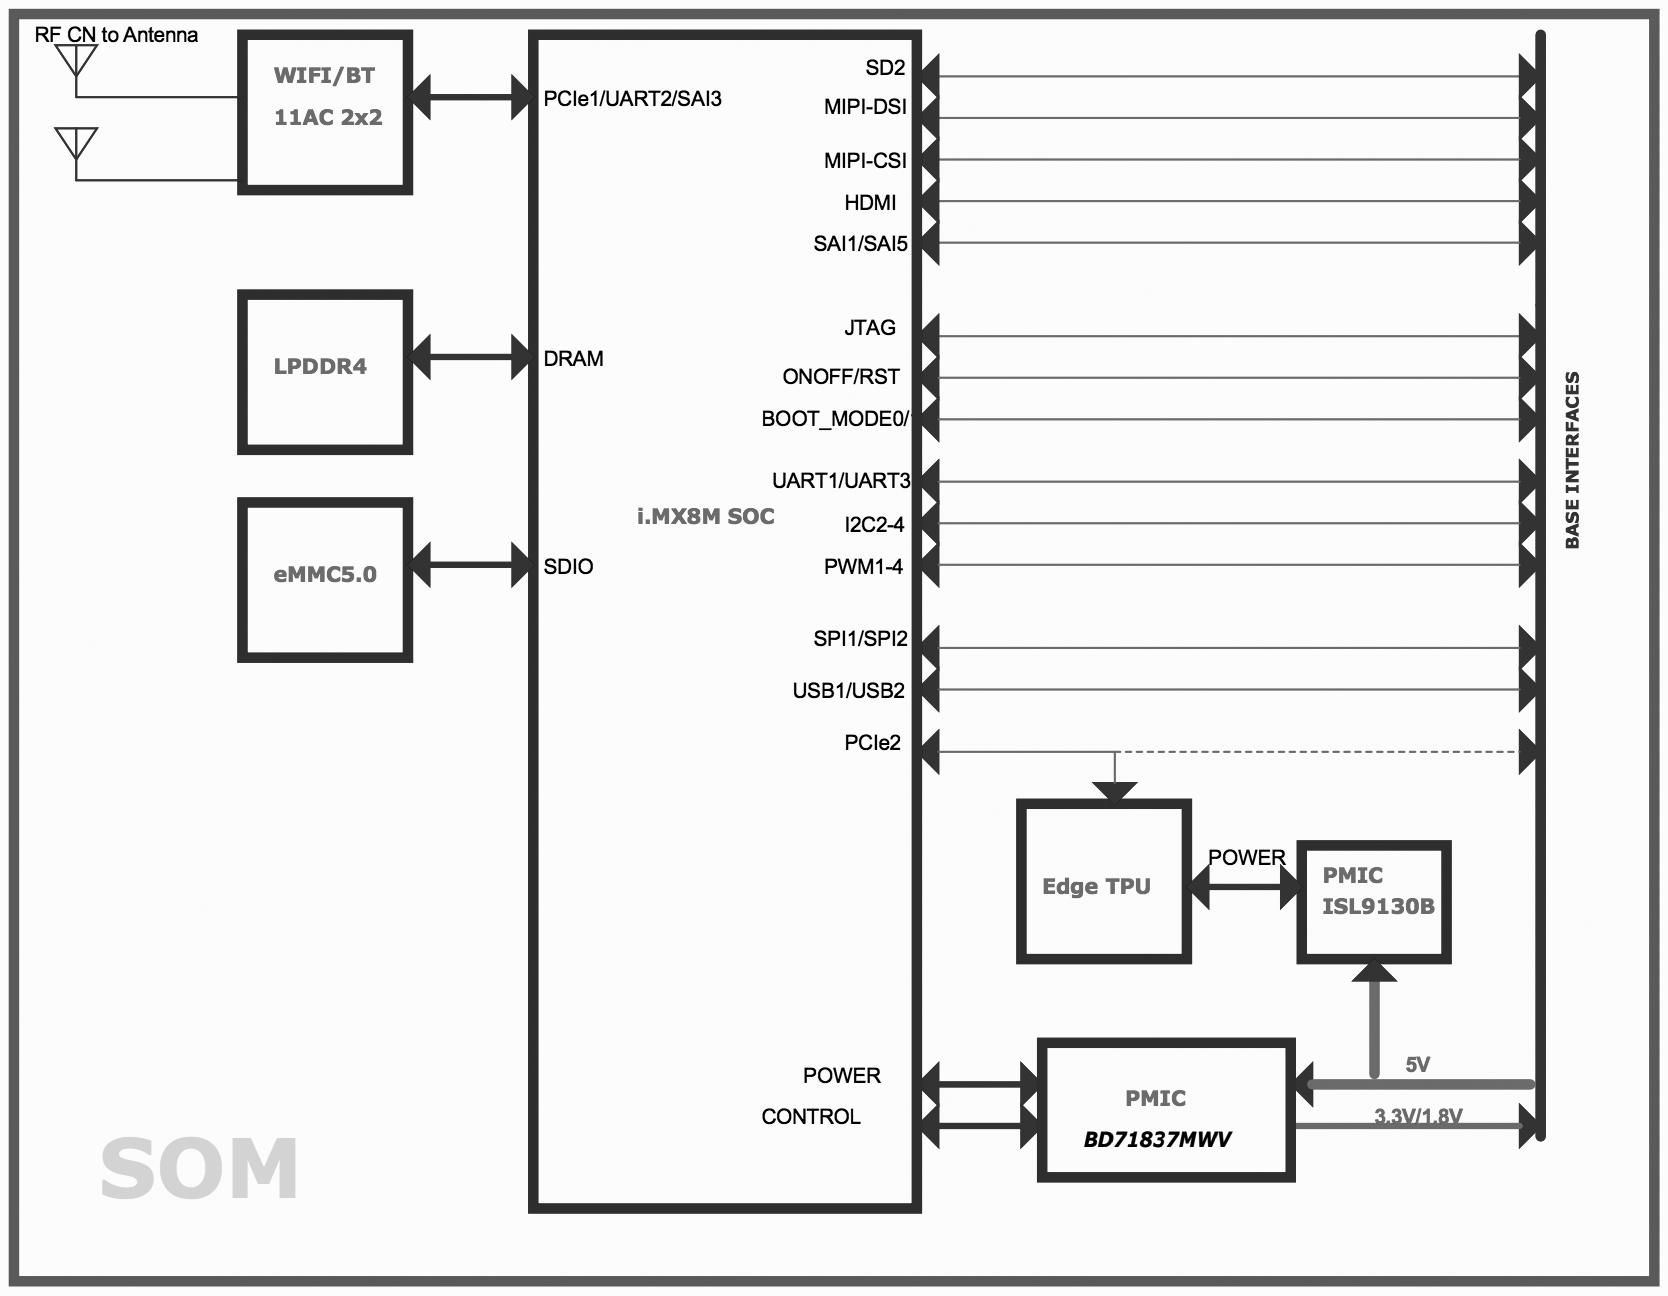
\includegraphics[scale=0.2]{../pdf/coral.png}
        \caption{Coral开发板SoM架构图}
        \label{coral}
    \end{figure}
    从图\ref{coral}可以看出,Coral架构中采用了NXP的i.MX8 SoC与Google研发的TPU模块通过PCIe2总线进行通信,二者组成异构计算平台,计算性能远超树莓派。

    本文通过研究Eyeriss架构,针对IoT领域,综合考虑算力、能耗、成本,开发一套基于异构处理器的用于图像识别的CNN计算加速系统。

\section{国内外发展现状}
    从 2015 年开始,AI 芯片的相关研发逐渐成为学术界和工业界研发的热点。到目前为止,在云端和终端已经有很多专门为 AI 应用设计的芯片和硬件系统。
    针对需求,目标应用可以划分为“ 训练”或者“推断”,目前在边缘 / 嵌入设备中以推断应用为主,
    训练的需求还不是很明确。有些高性能的边缘设备虽然也会进行训练,但从硬件本身来说,它们更类似于云端设备。
    未来的边缘和嵌入设备可能都需要具备一定的学习能力,以支持在线学习功能。

    文献[2]作者考虑到性能、功耗、灵活性,认为在嵌入式领域基于FPGA的DNN加速器是较为明智的选择。但是FPGA开发相对于软件开发更加困难,因此其提出了一种名为FP-DNN (FieldProgrammable DNN)的端到端框架。该框架使用TensorFlow描述的DNN作为输入,然后自动生成RTL-HLS混合的模板。文献[3]同样基于高层次方法的设计,方法与文献[2]大同小异。其实验数据表明性能是CPU的17.65倍。
    以上两篇文献设计方法是从高级语言框架(Tensorflow、Caffe等)入手,经过开发的编译器或者HLS技术映射到FPGA中,这种方法具有硬件开发周期短、工作量少的优势,但由于编译器和HLS技术的不完善,从高级语言编译出的RTL电路缺乏对硬件潜在的并行特性的开发,无法完全发挥出硬件电路的优势。
    文献[4]给出了另一种FPGA实现DNN的途径。其构造了一个DLAU (Deep Learning Accelerator Unit),该单元是一个可扩展DNN计算加速器,内含三级流水线,极大提高了数据吞吐量,其测试数据表明此方案比Intel双核处理器加速了36.1倍。这种设计方法更加符合硬件工程师思维,同时性能更加优异,但是其开发难度较大,且需要自行构造一些自动化工具来进行DNN系统配置。文献[5]给出了一种玻尔兹曼机的高性能FPGA实现,玻尔兹曼机可以理解为神经网络中的一个神经单元,文中描述软件实现的神经网络其复杂度是O(n2)级别,因此其无法提供非学术的性能和扩展性。文献作者充分利用了硬件潜在的并行特性构造的受限玻尔兹曼机将复杂度降低为O(n)级别,同时仅仅需要O(n)级别的资源。根据其在Xilinx Virtex II-Pro XC2VP70 上的测试,其可运行在100MHz频率,比2.8GHz的Intel处理器加速了35倍。
    现如今AI芯片的开发尚未出现标准的方法学,两种主流方案,其一是基于当前发展成熟的深度学习框架,将使用高级语言编写的DNN系统翻译成RTL电路,该方案开发周期短,且开发较为容易,但受限于编译器的缺陷,没有完全发挥硬件电路的特性;其二是构造一可扩展的单个神经元并配合自动化脚本,生成所需的DNN系统,该方案开发难度较大,但可以充分发挥硬件的特性,性能更加优秀。

\section{论文的主要研究内容及意义}
    本文主要基于文献[X]的思想,结合近几年发展起来的敏捷型HDL开发语言——Chisel,编写一款PE阵列生成器,可配置阵列大小、计算位宽、FIFO深度来满足不同神经网络的需要,
    结合异构处理器,完成对CNN的加速推断。

    同时,本课题对比了传统数字电路开发方法与敏捷型数字电路开发方法的优劣,探讨了基于敏捷型开发方法的流程。在新方法的框架下完成CNN加速系统加速器部分的开发。并通过Xilinx Vivado集成开发环境,完成系统的性能评估。
    运行一量化的手写数字识别网络,完成对系统的逻辑功能验证。

    本课题一方面可以帮助数字电路开发人员直观的比较传统Verilog与新型Chisel两种HDL语言的区别,方便对新技术有个全面的认识,另一方面构造的PE阵列生成器,可以十分方便的生成所需的规模,加速对不同AI应用场景加速系统的开发流程。

\section{论文章节安排}
    结合国内外发展现状,利用Chisel语言的特性,确定了基于异构处理器图像识别系统的需求设计,本文工作安排如下:

    第一章:绪论。本章简单介绍了当下国内外针对AI推断加速的主要成果以及主要研究内容和意义

    第二章:开发工具及相关技术介绍。本章首先简单介绍了基于JVM的Scala语言及其特性,随后重点介绍了基于Scala语言开发的Chisel语言的特性、使用方法、与Verilog的区别、开发流程。
    同时介绍了Verilator——一个开源、高性能的Verilog仿真工具。其次介绍了当前主流的两种异构处理器架构或平台,RISC-V和ZYNQ。最后介绍了神经网络在图像识别领域的典型应用和案例。

    第三章:系统功能需求分析与系统架构设计。本章首先介绍了传统架构和异构的优劣势,随后针对第二章介绍了两个异构平台设计了两种针对图像识别领域的CNN加速系统,其次简单描述了一下采用HLS与HDL两种开发的优劣,其中引出了敏捷型开发思想。
    最后详细介绍了在异构平台上计算任务的划分方法,以及基于行静止思想的卷积计算方法。
    
    第四章:硬件模块介绍。本章详细介绍了每一个PE阵列中使用的模块的引脚、功能、内部结构设计。最后详细介绍了充分发挥Chisel特性的PE阵列生成器的代码结构,以及其可配置参数的功能

    第五章:功能仿真结果。本章主要介绍了单个PE的仿真波形,详细介绍了每个阶段的关键信号以及逻辑行为,其次对一个6×7PE阵列的4D卷积计算波形图,并给出了综合实现之后的资源使用报告和时序报告。

    第六章:板级测试结果。本章基于PYNQ平台,集成开发的PE阵列开发了一个用于测试的板级系统,展示了基于一个int8量化的MNIST网络的实际运行结果。

% \subsection{二级节标题}

% \subsubsection{三级节标题}

% \paragraph{四级节标题}

% \subparagraph{五级节标题}

% \section{脚注}

% Lorem ipsum dolor sit amet, consectetur adipiscing elit, sed do eiusmod tempor
% incididunt ut labore et dolore magna aliqua. Ut enim ad minim veniam, quis
% nostrud exercitation ullamco laboris nisi ut aliquip ex ea commodo consequat.
% Duis aute irure dolor in reprehenderit in voluptate velit esse cillum dolore eu
% fugiat nulla pariatur. Excepteur sint occaecat cupidatat non proident, sunt in
% culpa qui officia deserunt mollit anim id est laborum.
% \footnote{This is a long long long long long long long long long long long long
% long long long long long long long long long long footnote.}

\chapter{开发工具及相关技术介绍}

\section{开发工具介绍}
    \subsection{Scala}
        Scala(Scalable Language)是一门多范式的编程语言,集成了面向对象编程、函数式编程和命令式编程的各种特性,同时该语言基于JVM,兼容Java编写的工具包,同时其内置的静态类型极大程度上降低了构建高性能系统的难度,是一门十分灵活、高级的编程语言。
        Scala自2004年被设计出来以后不断发展壮大,截止2019年2月已经发展到2.12.8版本,社区十分活跃,功能十分强大,不断的被大厂应用于产品:
        \begin{itemize}[topsep = 0 pt]
            \setlength{\topsep}{0pt}
            \setlength{\itemsep}{0pt}
            \setlength{\parsep}{0pt}
            \setlength{\parskip}{0pt}
            \setlength{\partopsep}{0pt}
            \item  Twitter宣布他们已经把大部分后端程序从Ruby迁移到Scala
            \item  Wattzon已经公开宣称,其整个平台都已经是基于Scala基础设施编写的
            \item  瑞银集团把Scala用于一般产品中
            \item  Coursera把Scala作为服务器语言使用
            \item  由UCB开发的大数据集群计算平台——Spark使用Scala作为开发语言
        \end{itemize}       
        \begin{lstlisting}[title=Scala Hello world, frame=shadowbox]
object HelloWorld {
    def main(args: Array[String]) {
        println("Hello, world!")
    }
}
        \end{lstlisting}

    \subsection{Chisel3}
        Chisel是一款由UC Berkeley开发并开源的硬件描述语言,支持高度参数化的生成器和分层设计等高级设计方法进行硬件设计。
        需要说明的是Chisel并不是将C转换成RTL(类似HLS),而是货真价实的硬件描述语言。其本身作为工具包内嵌于Scala中。 \\
        Chisel主要特性归纳如下:
        \begin{figure}[h]
            \begin{itemize}[topsep = 0 pt]
                \setlength{\topsep}{0pt}
                \setlength{\itemsep}{0pt}
                \setlength{\parsep}{0pt}
                \setlength{\parskip}{0pt}
                \setlength{\partopsep}{0pt}
                \item 支持抽象的数据类型和接口
                \item 批量连接
                \item 层次化、面向对象、函数式构造
                \item Scala元编程实现了高度参数化
                \item 内置了可配置的标准单元库
                \item 可生成Verilog
                \item 多时钟域设计
                \item 开源,完备的文档,活跃的社区
            \end{itemize}
        \end{figure}
        \begin{figure}[h]
            \label{chisel_example}
            \begin{lstlisting}[title=Chisel Example, frame=shadowbox]
import chisel3._
class MaxN(val n: Int, val w: Int) extends Module {
    private def Max2(x: UInt, y: UInt) = Mux(x > y, x, y)
    val io = IO(new Bundle {
        val ins = Input(Vec(n, UInt(w.W)))
        val out = Output(UInt(w.W))
    })
    io.out := io.ins.reduceLeft(Max2)
}
            \end{lstlisting}
        \end{figure}

    \subsection{Verilator}
Verilator是速度最快的Verilog HDL模拟器,性能优于大部分商用模拟器。其将Verilog转换为使用C++或SystemC编写的时序准确的模型。
\begin{wrapfigure}{r}{4cm}%靠文字内容的左侧
    
\includegraphics[width=4cm]{../pdf/verilator.png}\
    \caption{Verilator Logo}
\end{wrapfigure}
    Verilator专为需要快速仿真性能的大型项目而设计,尤其适用于为嵌入式软件设计团队生成可执行的CPU模型。其无法替代NC-Verilog,VCS等商业Verilog模拟器,但可以将可综合的Verilog迁移到C++或SystemC,并且是免费的。
Verilator的性能十分优秀,并不是将Verilog代码直接进行翻译而是优化为更快的线程区分模型。单线程的Verilator模型比传统Verilog仿真器(例如Icarus Verilog)快100倍,多线程可以获得额外的2倍~10倍性能。
目前Verilator已经用于仿真百万级门电路的设计中,并且被很多IP厂商支持,包括ARM和RISC-V。\\
其中Verilator官方网站给出一些与主流仿真器速度比较参考。
        \begin{itemize}[topsep = 0 pt]
            \setlength{\topsep}{0pt}
            \setlength{\itemsep}{0pt}
            \setlength{\parsep}{0pt}
            \setlength{\parskip}{0pt}
            \setlength{\partopsep}{0pt}
            \item Verilator比Icarus Verilog快90倍
            \item Verilator比ModelSim SE快10至40倍
            \item Verilator比NC-Verilog快3倍
            \item Verilator比VCS快1.5倍
        \end{itemize}


\section{异构处理器}
    \subsection{ZYNQ架构}
    ZYNQ是Xilinx于2010年4月发布的可扩展架构平台,该平台基于流行的ARM处理器结合Xilinx 28nm 7系FPGA工艺打造的SoC实现了高度的灵活性、强大的配置性和高特性的统一。
    其中可编程逻辑可由用户配置,并通过互联模块连接,可为用户提供自定义的逻辑,从而极大扩展了处理系统的性能和功能,不过和传统FPGA不同,ZYNQ不仅可以在开机时配置也可以根据需要实时进行配置。
    \begin{figure}[h]
        \label{zynq}
        \centering
        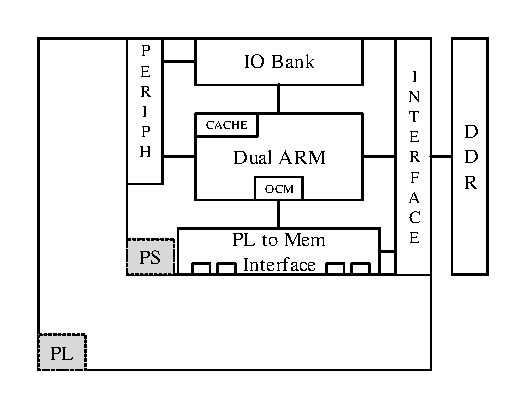
\includegraphics{../pdf/zynq.pdf}
        \caption{ZYNQ架构示意图}
        \label{}
    \end{figure}
    ZYNQ由于CPU+FPGA的架构十分契合异构计算的需求,同时PS与PL之间可以通过设计好的高带宽的AXI接口进行数据交互,开发者只需将精力集中在加速器设计和CPU数据调度上即可。
    \subsection{RISC-V}
    RISC-V从伯克利大学诞生的一款开源指令集架构,引起业界的轰动,普遍认为RISC-V可能会改变现有的由ARM、x86主导的处理器市场竞争格局。

    由于RISC-V是新的指令集架构,因此无需考虑向前兼容,没有像ARM、x86架构沉重的历史包袱,指令集的设计也更加精简。

    \begin{table}[h] %开始一个表格environment,表格的位置是h,here。  
        \label{riscv_compare}
        \centering
        \caption{RISC-V与ARM/x86比较} %显示表格的标题  
        \begin{tabular}{l|l|l} %设置了每一列的宽度,强制转换。  
        \hline  
        特性 & ARM/x86 & RISC-V \\
        \hline %画一个横线,下面的就都是一样了,这里一共有4行内容  
        架构篇幅 & 数千页  & 目前仅有300页 \\
        \hline  
        模块化 & 不支持  & 支持模块化可配置指令子集 \\
        \hline  
        可扩展性 & 不支持 & 支持扩展自定义指令 \\
        \hline  
        指令数目 & 指令多且不同分支不兼容 & 一套指令支持所有架构分支,基本指令仅40条 \\
        % \hline  
        % 易实现性 & 硬件实现十分复杂 &  \\
        \hline  
        \end{tabular}  
    \end{table}

    由伯克利大学维护的一款开源RISC-V芯片生成器Rocket-Chip-Generator,能够根据用户需要生成完整的、可综合的硬件电路,同时具备完整的工具链、准确的仿真器环境,目前已被各大厂商应用。

    \begin{figure}[h]
        \label{rocc}
        \centering
        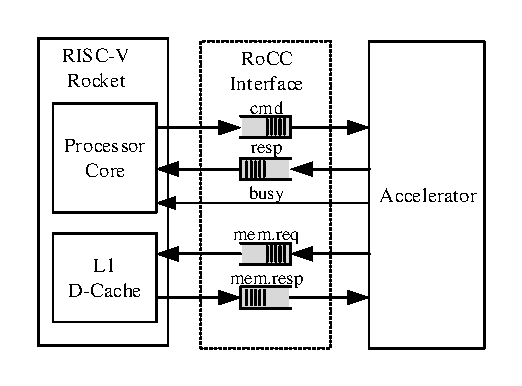
\includegraphics{../pdf/rocc.pdf}
        \caption{RoCC接口信号示意图}
        \label{}
    \end{figure}

    Rocket-Chip原生支持自定义指令集扩展,其带有一RoCC(Rocket Custom Coprocessor)接口,其协议简单、功能强大,可以十分灵活的以自定义加速器进行协同工作。


\section{深度学习}
    \subsection{YOLO}
    YOLO(You only look once)是一个端到端的实时目标检测算法,不像传统的目标识别CNN模型需要训练多个分类器之后在图像上使用滑动窗的形式进行检测,YOLO会在整张图片上进行卷积进行目标识别工作,就像它名字所说,YOLO只需看一次图片即可,
    因此极大的缩短了计算时间,提高了实时性
    目前YOLO已经推出了三个版本,因其识别效果十分显著,已经被各大厂商应用在各自领域。
    \begin{figure}[h]
        \centering
        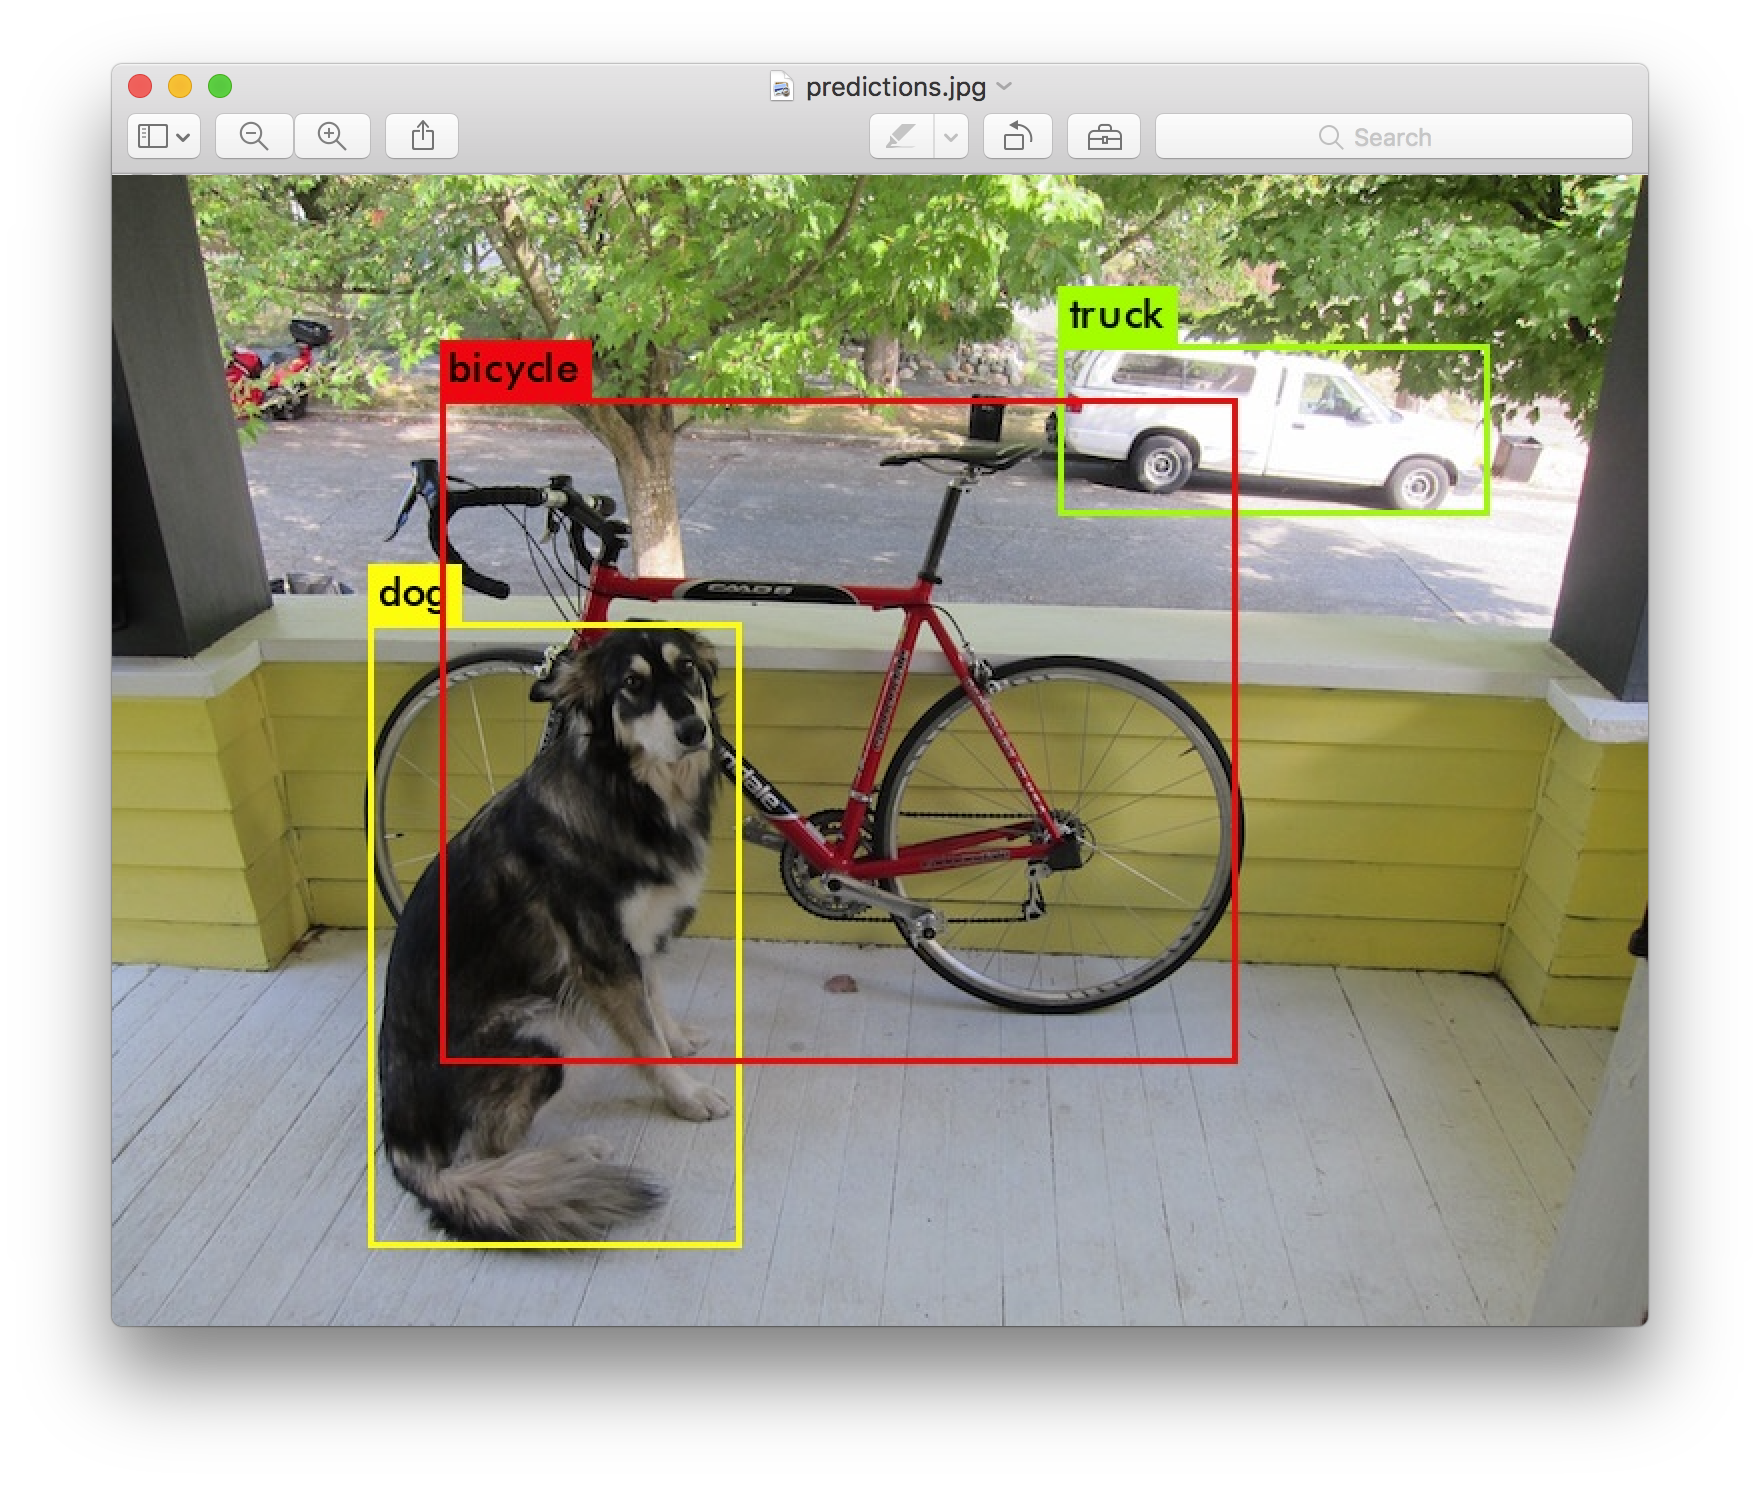
\includegraphics[scale=0.2]{../pdf/yolo.png}
        \caption{YOLO效果图}
        \label{}
    \end{figure}
    \subsection{LeNet-5}
    LeNet-5是一种用于手写体识别的卷积神经网络,是CNN领域五大经典模型之一。该网络虽小,但包含了深度学习的基本模块,如卷积层、池化层、全连接层,是其他CNN模型的基础。
    \begin{table}[h] %开始一个表格environment,表格的位置是h,here。  
        \centering
        \caption{LeNet-5 模型结构} %显示表格的标题  
        \begin{tabular}{l|l} %设置了每一列的宽度,强制转换。  
        \hline  
        Lenet-5 layers & 描述 \\
        \hline %画一个横线,下面的就都是一样了,这里一共有4行内容  
        Layer1[Conv] & Input: $32*32*1$ \  Filter: $5*5*6, stride=1$ \  Output: $28*28*6$ \\
        \hline  
        Layer2[Pooling] & Input: $28*28*6$ \  Filter: $2*2*6, stride=2$ \  Output: $14*14*6$ \\
        \hline  
        Layer3[Conv] & Input: $14*14*6$ \  Filter: $5*5*16, stride=1$ \  Output: $10*10*16$ \\
        \hline  
        Layer4[Pooling] & Input: $10*10*16$ \  Filter: $2*2*16, stride=2$ \  Output: $5*5*16$ \\
        \hline  
        Layer5[Fully Connect] & $400*120$ \\
        \hline  
        Layer6[Fully Connect] & $120*84$ \\
        \hline  
        Layer7[Fully Connect] & $84*10$  \\
        \hline  
        \end{tabular}  
    \end{table}


\section{本章小结}
本章首先对采用的开发工具进行了简要的阐述,其次举例介绍了目前使用较为广泛的异构处理器ZYNQ和RISC-V,最后介绍了利用CNN进行目标识别和图像识别的典型网络。

% \subsection{二级节标题}

% \subsubsection{三级节标题}

% \paragraph{四级节标题}

% \subparagraph{五级节标题}

% \section{脚注}

% Lorem ipsum dolor sit amet, consectetur adipiscing elit, sed do eiusmod tempor
% incididunt ut labore et dolore magna aliqua. Ut enim ad minim veniam, quis
% nostrud exercitation ullamco laboris nisi ut aliquip ex ea commodo consequat.
% Duis aute irure dolor in reprehenderit in voluptate velit esse cillum dolore eu
% fugiat nulla pariatur. Excepteur sint occaecat cupidatat non proident, sunt in
% culpa qui officia deserunt mollit anim id est laborum.
% \footnote{This is a long long long long long long long long long long long long
% long long long long long long long long long long footnote.}

\chapter{系统功能需求分析与系统架构设计}

\section{系统功能需求}
文献X中表明,在一确定的CNN中,卷积的计算时间占据了至少85\%,因此若想制作一款CNN加速器,那么急需解决的问题就是如何加速图像的卷积计算。
卷积计算虽然参数相比于CNN中全连接层少,但其计算量非常大,而且通常为简单的乘加操作。
    \subsection{传统架构}
        \subsubsection{CPU}
        首先,CPU在深度学习计算中很重要,例如使用了16000颗CPU搭建的“Google Brain”网络,又比如1920颗CPU搭建的“AlphaGo”。如今,CPU依旧是主流深度学习平台的重要组成部分,
        但在深度学习领域,CPU在架构方面有着先天的不足,从芯片面积上看,Cache和Control单元占据了绝大部分面积,而用于计算的ALU面积却比较少;每颗核心都狠强大,但核心数量少。
        因此CPU重在数据调度,并不擅长大规模简单的运算。
        \subsubsection{GPU}
        反观GPU,虽然每颗核心都比较弱,只能完成简单的计算,但通常一个GPU都是上百上千个核心,芯片面积上用于计算的ALU单元占据了绝大部分,当所有核心都被调用起来,其运算能力远远大于CPU。
        同时,GPU普遍采用DDR5片上显存颗粒,更高的工作频率带来了更快的数据读写速度,而且总线带宽大。
    \subsection{异构的优势}
        目前做深度学习开发普遍采用CPU+GPU这种异构形式作为首要开发平台,既可以利用CPU强大的调度能力也可以利用GPU超快的计算速度,但这种模式是一种通用级的解决方法,应用在细分的专业领域边显的过于臃肿,不仅设备体积大,功耗也高。
        一般情况下,当模型训练完成后,需要利用模型进行推理计算,这部分不需要复杂的反向传播计算,若继续采用训练时的CPU+GPU平台,不仅造成资源浪费,量产时成本极高。
        因此针对推断,我们希望能找到一种低功耗、高性能的解决方案,因此使用FPGA和ASIC具有极大的优势。

        相比于通用的CPU+GPU的架构,CPU+FPGA/ASIC组成的异构平台具有更高的计算能效比,同时成本更低,十分适合当下嵌入式IoT领域对低功耗、高灵活性的需求。
        相比于受限于冯诺依曼架构的CPU/GPU,FPGA和ASIC在设计时可以通过多核心、流水线等技术充分发挥并行计算的特性,大大提高数据吞吐量。

\section{系统架构设计}
    针对本章第一节的需求,本文通过调研当前硬件加速方案,参考论文X的思想设计了一套针对CNN计算加速的方案。
    \begin{figure}[h]
        \centering
        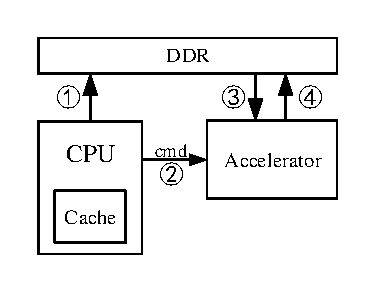
\includegraphics{../pdf/system.pdf}
        \caption{CNN加速系统架构示意图}
        \label{}
    \end{figure}

\section{开发环境}
    \subsection{HLS}
    HLS(High Level Synthesis)也既高层次综合技术,是Xilinx公司大力推广的一项FPGA开发技术。该技术使用C/C++作为开发语言,可以充分利用该语言中提供的数据结构进行FPGA开发。
    最终可以生成Verilog或VHDL语言。

    通过HLS使得软件工程师可以不用了解FPGA和Verilog,也可以使用FPGA进行硬件加速,大幅减少FPGA开发难度和开发周期。该技术已应用在SDAccel、SDSoC等软件中,目前在偏算法的视频图像处理领域有着广泛的应用。

    但简单易用的东西背后都会带来不必要的性能浪费。与传统HDL开发相比,HLS无法对电路进行精细化操作,因此虽然HLS能够大大缩短开发周期,但从能性能方面传统HDL开发更具有优势。
    \subsection{OpenCL}
    HLS可以进行算法的快速实现,但是并不适合大规模系统开发。OpenCL的出现给人们带来使用高层次综合进行大规模系统开发的希望。
    OpenCL(Open Computing Language)即开放运算语言,是第一个面向异构系统通用目的并行编程的开放式、免费标准,也是一个统一的编程环境,广泛使用于CPU,GPU,DSP,FPGA等并行处理器的开发。
    其提供了一系统采用C/C++封装的API,编写的程序可以在支持OpenCL的设备上运行。
    与HLS相似,OpenCL也使开发人员脱离底层电路,允许在系统层面进行开发。由于OpenCL是跨平台的,因此可以很容易的将原来CPU或GPU的代码做些许改动就能在支持OpenCL的FPGA上运行。
    \subsection{敏捷型开发}
    敏捷型开发思想源于软件工程,其宗旨是以用户需求进化为核心,采用迭代、循序渐进的方法进行软件开发,在此过程中软件一直处于可工作状态。软件之所以可以采用敏捷型开发是因为其反馈环足够短,同时软件开发工具成熟易用。
    而目前数字芯片公司大多对敏捷性开发很陌生,事实上芯片开发周期长已经是阻碍数字芯片设计快速发展的重要瓶颈。传统数字芯片公司大多采用Verilog的同时,还需使用一些非标准的Python/Perl等脚本语言进行代码编写自动化任务,
    而然这种方式可移植性差,同时调试比较困难。
    \begin{figure}[h]
        \centering
        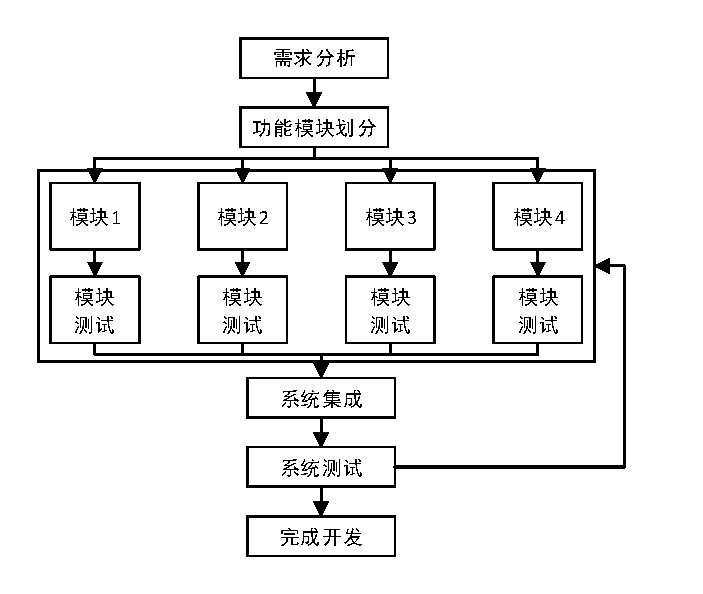
\includegraphics{../pdf/tradition.pdf}\\
        \caption{传统开发流程图}
        \label{tra}
    \end{figure}
    \begin{figure}[h]
        \centering
        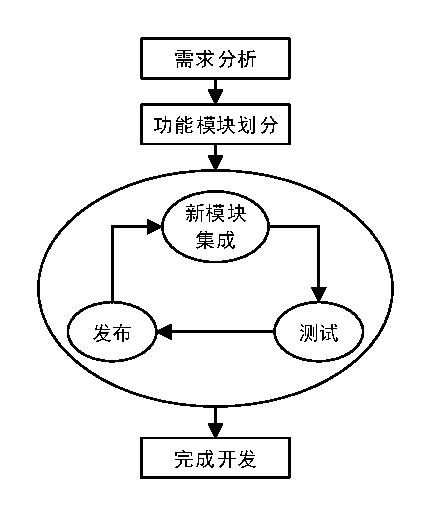
\includegraphics{../pdf/agile.pdf}\\
        \caption{敏捷型开发流程图}
        \label{agi}
    \end{figure}
    传统的开发流程可以参考图\ref{tra},可以发现开发流程呈线性,当前阶段完成后只需关注后续阶段,但用户只有等到整个过程末期才能见到开发效果,增加了开发风险,同时灵活性较低。
    敏捷型开发流程可以参考图\ref{agi},其主要开发过程呈现环状,当发布第一版之后便可见到项目雏形,同时具有高适应性可以随着开发深入遇见的问题随时调整方向。

\section{基于行静止思想的卷积计算方法}
如本章第二节所述,计划采用CPU+FPGA实现卷积神经网络的计算加速。
\begin{figure}[h]
    \centering
    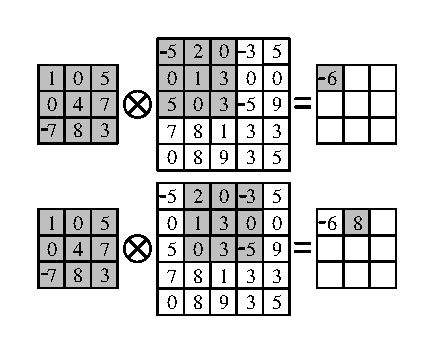
\includegraphics{../pdf/tra_conv.pdf}\\
    \caption{图像卷积计算流程}
    \label{tra_conv}
\end{figure}
传统图像卷积计算流程如图\ref{tra_conv} 所示,卷积核先与图像第一行第一列开始的同等大小矩阵进行点乘运算,计算结果进行累加得到结果的第一个值,然后卷积核在图像上向右进行滑动,再次进行点乘累加运算即可得到第二个值。
通过滑动卷积核,即可得到整张图片的卷积结果。
\begin{figure}[h]
    \centering
    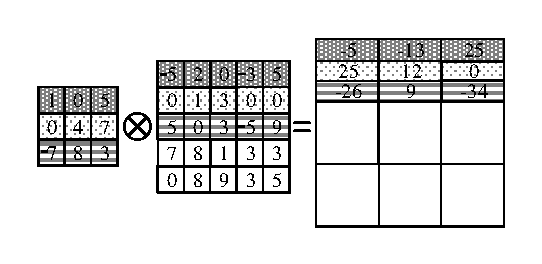
\includegraphics{../pdf/row_conv.pdf}\\
    \caption{行静止卷积计算流程}
    \label{row_conv}
\end{figure}
基于行静止思想的卷积的计算模式如图\ref{row_conv} 所示,其与普通的卷积计算模式不同,首先卷积核的第一行和图像的第一行进行一维卷积操作(图中阴影背景所标出的部分),计算结果进行缓存。
之后卷积核第二行和图像的第二行进行一维卷积操作(图中斑点背景标出部分),卷积结果和上一次按位置进行累加。
最后卷积核和图像的第三行进行一维卷积计算,得到的结果再次进行按位置累加操作,即可得到最终结果的第一行。
然后卷积核的第一、二、三行分别于图像的二、三、四行进行一维卷积操作,即可得到最终结果的第二行。
通过迭代此过程即可得到完整的卷积结果。

这种计算模式虽然不能减少计算次数,但是十分适合硬件去进行数据缓存以减少与DDR进行交互的能量消耗。



\section{本章小结}

% \subsection{二级节标题}

% \subsubsection{三级节标题}

% \paragraph{四级节标题}

% \subparagraph{五级节标题}

% \section{脚注}

% Lorem ipsum dolor sit amet, consectetur adipiscing elit, sed do eiusmod tempor
% incididunt ut labore et dolore magna aliqua. Ut enim ad minim veniam, quis
% nostrud exercitation ullamco laboris nisi ut aliquip ex ea commodo consequat.
% Duis aute irure dolor in reprehenderit in voluptate velit esse cillum dolore eu
% fugiat nulla pariatur. Excepteur sint occaecat cupidatat non proident, sunt in
% culpa qui officia deserunt mollit anim id est laborum.
% \footnote{This is a long long long long long long long long long long long long
% long long long long long long long long long long footnote.}

\chapter{硬件模块介绍}

\section{基于FIFO的可变长移位寄存器设计}

\begin{figure}[h]
    \centering
    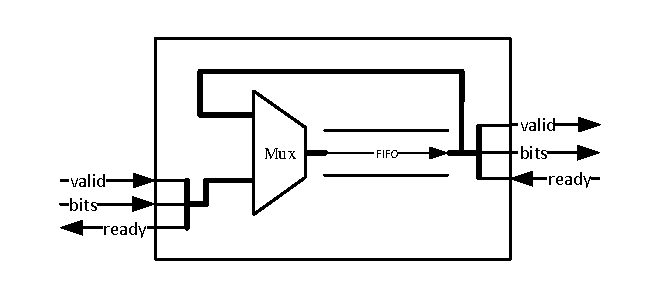
\includegraphics{../pdf/fifoshift.pdf}\\
    \caption{FIFO Shift}
\end{figure}
利用FIFO的先入先出特性,配合外部控制信号可以构造一个最大位宽为FIFO深度的移位寄存器。
首先,模块中的Mux将FIFO接口入模块输入信号连接,此时数据被写入FIFO中,当数据输入过程完成之后,Mux将模块内的FIFO输入与输出对接,
此时便形成了一个数据环路,FIFO输出的数据被输入给FIFO的输入,使数据一直保留在FIFO中。

实际使用时,FIFO深度被配置为256,位宽为16bit。第一阶段,FIFO输入通过Mux与模块的输入对接,接受来自外部的图像或者卷积核信息,第一阶段取数完成后进入第二阶段——计算,此时FIFO的输入与FIFO的输出对接,吐出的数据再次被存入FIFO中,以达到移位寄存器的功能。

需要说明的是,,该构造读数时每次只能读取最末端的数据,

    \subsection{BRAM与DRAM选择}

\section{SRAM部分在FPGA中的优化}

\section{基于Xilixn 7Series FPGA片上DSP的高性能乘法器}

\section{PE单元构造}

\section{用于数据分发的简易NoC设计}

\section{PE阵列生成器}
    \subsection{计算流程}

\section{顶层接口设计}

\section{本章小结}
% \subsection{二级节标题}

% \subsubsection{三级节标题}

% \paragraph{四级节标题}

% \subparagraph{五级节标题}

% \section{脚注}

% Lorem ipsum dolor sit amet, consectetur adipiscing elit, sed do eiusmod tempor
% incididunt ut labore et dolore magna aliqua. Ut enim ad minim veniam, quis
% nostrud exercitation ullamco laboris nisi ut aliquip ex ea commodo consequat.
% Duis aute irure dolor in reprehenderit in voluptate velit esse cillum dolore eu
% fugiat nulla pariatur. Excepteur sint occaecat cupidatat non proident, sunt in
% culpa qui officia deserunt mollit anim id est laborum.
% \footnote{This is a long long long long long long long long long long long long
% long long long long long long long long long long footnote.}

\chapter{功能仿真结果}

\section{利用Chisel3配套工具进行快速仿真}
Chisel3在Github网站上有一套基于Scala体系的仿真工具,chisel-testers。
使用该工具可以直接在Scala中实例化使用Chisel3开发的模块,并且产生激励进行模块的仿真。
其主要提供了一个名为PeekPokeTester的类,该类提供了能够完成激励产生和信号断言的方法。
\begin{table}[h] %开始一个表格environment,表格的位置是h,here。  
    \centering
    \caption{PeekPokeTester中提供的方法} %显示表格的标题  
    \begin{tabular}{l|l|c} %设置了每一列的宽度,强制转换。  
    \hline  
    \hline  
    方法名 & 作用 & 使用举例 \\ %用&来分隔单元格的内容 \\表示进入下一行  
    \hline %画一个横线,下面的就都是一样了,这里一共有4行内容  
    poke & 设置DUT的输入信号 & poke(c.io.in.valid, 1) \\
    \hline  
    peek & 读取DUT的输出信号 & peek(c.io.out.bits) \\
    \hline  
    expect & 比较DUT的输出信号 & expect(c.io.out.bit, 0xff) \\
    \hline  
    step & 驱动DUT的时钟信号 & step(1) \\
    \hline
    reset & 驱动DUT的复位信号 & reset(1) \\
    \hline  
    \hline  
    \end{tabular}  
\end{table}
同时,该工具支持使用Verilator作为仿真后端,大大降低了大规模电路的仿真时间,借助Verilator,可以产生仿真时的vcd仿真文件,通过GTKWave、Verdi等波形查看工具即可查看仿真波形,
使用时十分便利。
            \begin{lstlisting}[title=Chisel Test Example, frame=shadowbox]
class Tester(c: Test) extends PeekPokeTester(c) {
  poke(c.io.in, -1)     //Set DUT input "in" as -1
  step(1)               //wait 1 clock
  expect(c.io.out, -1)  //assert DUT output "out" as -1
}
            \end{lstlisting}

\section{基于FIFO的可变长移位寄存器仿真结果}
% filters: DenseVector(0, 2, -1) __ 3
% filterNum: 1
% imgs: DenseVector(4, -3, -3, -1, -5) __ 5
% imgNum: 1
% nchannel: 1
\begin{figure}[h]
    \centering
    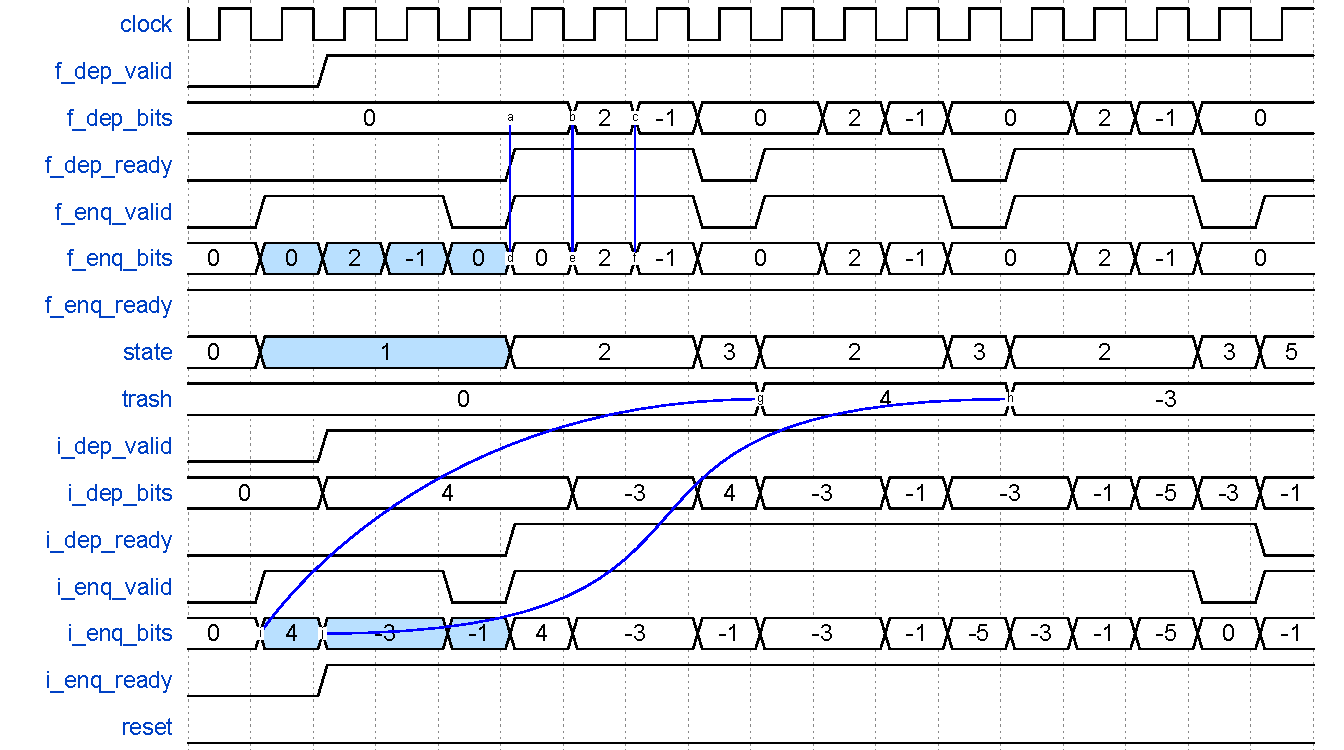
\includegraphics[scale=0.7]{../pdf/shift_w.pdf}\\
    \caption{SRAM IP波形图}
\end{figure}

\section{Designware SRAM IP仿真结果}
\begin{figure}[h]
    \centering
    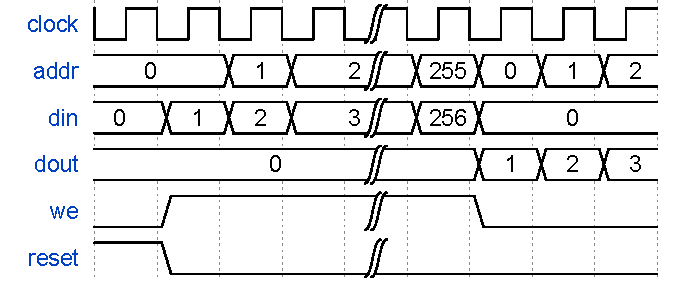
\includegraphics{../pdf/sram_w.pdf}\\
    \caption{SRAM IP波形图}
\end{figure}

\section{PE单元仿真结果}

\section{PE阵列仿真结果}

\section{运行MNIST测试结果}
    \subsection{模型量化}
    \subsection{运行流程}
    \subsection{输出结果与数学结果映射关系}

\section{系统性能}
    \subsection{资源占用}
    \subsection{时序报告}

\section{本章小结}
% \subsection{二级节标题}

% \subsubsection{三级节标题}

% \paragraph{四级节标题}

% \subparagraph{五级节标题}

% \section{脚注}

% Lorem ipsum dolor sit amet, consectetur adipiscing elit, sed do eiusmod tempor
% incididunt ut labore et dolore magna aliqua. Ut enim ad minim veniam, quis
% nostrud exercitation ullamco laboris nisi ut aliquip ex ea commodo consequat.
% Duis aute irure dolor in reprehenderit in voluptate velit esse cillum dolore eu
% fugiat nulla pariatur. Excepteur sint occaecat cupidatat non proident, sunt in
% culpa qui officia deserunt mollit anim id est laborum.
% \footnote{This is a long long long long long long long long long long long long
% long long long long long long long long long long footnote.}

\chapter{板级测试结果}

\section{PYNQ}

\section{用于测试的SoC系统}

\section{运行结果}

\section{本章小结}
% \subsection{二级节标题}

% \subsubsection{三级节标题}

% \paragraph{四级节标题}

% \subparagraph{五级节标题}

% \section{脚注}

% Lorem ipsum dolor sit amet, consectetur adipiscing elit, sed do eiusmod tempor
% incididunt ut labore et dolore magna aliqua. Ut enim ad minim veniam, quis
% nostrud exercitation ullamco laboris nisi ut aliquip ex ea commodo consequat.
% Duis aute irure dolor in reprehenderit in voluptate velit esse cillum dolore eu
% fugiat nulla pariatur. Excepteur sint occaecat cupidatat non proident, sunt in
% culpa qui officia deserunt mollit anim id est laborum.
% \footnote{This is a long long long long long long long long long long long long
% long long long long long long long long long long footnote.}

\chapter{结论}

% \subsection{二级节标题}

% \subsubsection{三级节标题}

% \paragraph{四级节标题}

% \subparagraph{五级节标题}

% \section{脚注}

% Lorem ipsum dolor sit amet, consectetur adipiscing elit, sed do eiusmod tempor
% incididunt ut labore et dolore magna aliqua. Ut enim ad minim veniam, quis
% nostrud exercitation ullamco laboris nisi ut aliquip ex ea commodo consequat.
% Duis aute irure dolor in reprehenderit in voluptate velit esse cillum dolore eu
% fugiat nulla pariatur. Excepteur sint occaecat cupidatat non proident, sunt in
% culpa qui officia deserunt mollit anim id est laborum.
% \footnote{This is a long long long long long long long long long long long long
% long long long long long long long long long long footnote.}


% \chapter{数学}

\section{数学符号}

模板定义了一些正体(upright)的数学符号:
\begin{center}
\begin{tabular}{rl}
  \toprule
    符号                 & 命令 \\
  \midrule
    常数$\eu$     & \verb|\eu| \\
    复数单位$\iu$ & \verb|\iu| \\
    微分符号$\diff$ & \verb|\diff| \\
    $\argmax$         & \verb|\argmax| \\
    $\argmin$         & \verb|\argmin| \\
  \bottomrule
\end{tabular}
\end{center}

更多的例子:
\begin{equation}
  \eu^{\iu\pi} + 1 = 0
\end{equation}
\begin{equation}
  \frac{\diff^2u}{\diff t^2} = \int f(x) \diff x
\end{equation}
\begin{equation}
  \argmin_x f(x)
\end{equation}

\section{定理、引理和证明}

\begin{definition}
    If the integral of function $f$ is measurable and non-negative, we define
    its (extended) \textbf{Lebesgue integral} by
    \begin{equation}
        \int f = \sup_g \int g,
    \end{equation}
    where the supremum is taken over all measurable functions $g$ such that
    $0 \leq g \leq f$, and where $g$ is bounded and supported on a set of
    finite measure.
\end{definition}

\begin{example}
    Simple examples of functions on $\mathbb{R}^d$ that are integrable
    (or non-integrable) are given by
    \begin{equation}
        f_a(x) =
        \begin{cases}
            |x|^{-a} & \text{if } |x| \leq 1,\\
            0 & \text{if } x > 1.
        \end{cases}
    \end{equation}
    \begin{equation}
        F_a(x) = \frac{1}{1 + |x|^a}, \qquad \text{all } x \in \mathbb{R}^d.
    \end{equation}
    Then $f_a$ is integrable exactly when $a < d$, while $F_a$ is integrable
    exactly when $a > d$.
\end{example}

\begin{lemma}[Fatou]
    Suppose $\{f_n\}$ is a sequence of measurable functions with $f_n \geq 0$.
    If $\lim_{n \to \infty} f_n(x) = f(x)$ for a.e. $x$, then
    \begin{equation}
        \int f \leq \liminf_{n \to \infty} \int f_n.
    \end{equation}
\end{lemma}

\begin{remark}
    We do not exclude the cases $\int f = \infty$,
    or $\liminf_{n \to \infty} f_n = \infty$.
\end{remark}

\begin{corollary}
    Suppose $f$ is a non-negative measurable function, and $\{f_n\}$ a sequence
    of non-negative measurable functions with
    $f_n(x) \leq f(x)$ and $f_n(x) \to f(x)$ for almost every $x$. Then
    \begin{equation}
        \lim_{n \to \infty} \int f_n = \int f.
    \end{equation}
\end{corollary}

\begin{proposition}
    Suppose $f$ is integrable on $\mathbb{R}^d$. Then for every $\epsilon > 0$:
    \begin{enumerate}
        \renewcommand{\theenumi}{\roman{enumi}}
        \item There exists a set of finite measure $B$ (a ball, for example) such that
        \begin{equation}
            \int_{B^c} |f| < \epsilon.
        \end{equation}
        \item There is a $\delta > 0$ such that
        \begin{equation}
            \int_E |f| < \epsilon \qquad \text{whenever } m(E) < \delta.
        \end{equation}
    \end{enumerate}
\end{proposition}

\begin{theorem}
    Suppose $\{f_n\}$ is a sequence of measurable functions such that
    $f_n(x) \to f(x)$ a.e. $x$, as $n$ tends to infinity.
    If $|f_n(x)| \leq g(x)$, where $g$ is integrable, then
    \begin{equation}
        \int |f_n - f| \to 0 \qquad \text{as } n \to \infty,
    \end{equation}
    and consequently
    \begin{equation}
        \int f_n \to \int f \qquad \text{as } n \to \infty.
    \end{equation}
\end{theorem}

\begin{proof}
    Trivial.
\end{proof}



\section{自定义}

\newtheorem*{axiomofchoice}{Axiom of choice}
\begin{axiomofchoice}
    Suppose $E$ is a set and ${E_\alpha}$ is a collection of
    non-empty subsets of $E$. Then there is a function $\alpha
    \mapsto x_\alpha$ (a ``choice function'') such that
    \begin{equation}
        x_\alpha \in E_\alpha,\qquad \text{for all }\alpha.
    \end{equation}
\end{axiomofchoice}

\newtheorem{observation}{Observation}
\begin{observation}
    Suppose a partially ordered set $P$ has the property
    that every chain has an upper bound in $P$. Then the
    set $P$ contains at least one maximal element.
\end{observation}
\begin{proof}[A concise proof]
    Obvious.
\end{proof}

% \chapter{浮动体}

\section{三线表}

三线表是《撰写手册》推荐使用的方式,如表~\ref{tab:exampletable}。
\begin{table}[htbp]
  \centering
  \caption{这里是表的标题}
  \label{tab:exampletable}
  \begin{tabular}{cl}
    \toprule
      操作系统 & TeX 发行版 \\
    \midrule
      所有 & TeX Live \\
      macOS & MacTeX \\
      Windows & MikTeX \\
    \bottomrule
  \end{tabular}
  \note{一个很长长长长长长长长长长长长长长长长长长长长长长长长长长长长长长长长长
  长长长长长长长长长长长的表注。}
\end{table}



\section{长表格}

超过一页的表格要使用专门的 \texttt{longtable} 环境(表~\ref{tab:longtable})。
\begin{longtable}{ccc}
  % 首页表头
  \caption[长表格演示]{长表格演示}
  \label{tab:longtable}\\
  \toprule[1.5pt]
    名称  & 说明 & 备注\\
  \midrule[1pt]
  \endfirsthead
  % 续页表头
  \caption[]{长表格演示(续)} \\
  \toprule[1.5pt]
  名称  & 说明 & 备注 \\
  \midrule[1pt]
  \endhead
  % 首页表尾
  \hline
  \multicolumn{3}{r}{\small 续下页}
  \endfoot
  % 续页表尾
  \bottomrule[1.5pt]
  \endlastfoot

  AAAAAAAAAAAA   &   BBBBBBBBBBB   &   CCCCCCCCCCCCCC   \\
  AAAAAAAAAAAA   &   BBBBBBBBBBB   &   CCCCCCCCCCCCCC   \\
  AAAAAAAAAAAA   &   BBBBBBBBBBB   &   CCCCCCCCCCCCCC   \\
  AAAAAAAAAAAA   &   BBBBBBBBBBB   &   CCCCCCCCCCCCCC   \\
  AAAAAAAAAAAA   &   BBBBBBBBBBB   &   CCCCCCCCCCCCCC   \\
  AAAAAAAAAAAA   &   BBBBBBBBBBB   &   CCCCCCCCCCCCCC   \\
  AAAAAAAAAAAA   &   BBBBBBBBBBB   &   CCCCCCCCCCCCCC   \\
  AAAAAAAAAAAA   &   BBBBBBBBBBB   &   CCCCCCCCCCCCCC   \\
  AAAAAAAAAAAA   &   BBBBBBBBBBB   &   CCCCCCCCCCCCCC   \\
  AAAAAAAAAAAA   &   BBBBBBBBBBB   &   CCCCCCCCCCCCCC   \\
  AAAAAAAAAAAA   &   BBBBBBBBBBB   &   CCCCCCCCCCCCCC   \\
  AAAAAAAAAAAA   &   BBBBBBBBBBB   &   CCCCCCCCCCCCCC   \\
  AAAAAAAAAAAA   &   BBBBBBBBBBB   &   CCCCCCCCCCCCCC   \\
  AAAAAAAAAAAA   &   BBBBBBBBBBB   &   CCCCCCCCCCCCCC   \\
  AAAAAAAAAAAA   &   BBBBBBBBBBB   &   CCCCCCCCCCCCCC   \\
  AAAAAAAAAAAA   &   BBBBBBBBBBB   &   CCCCCCCCCCCCCC   \\
  AAAAAAAAAAAA   &   BBBBBBBBBBB   &   CCCCCCCCCCCCCC   \\
  AAAAAAAAAAAA   &   BBBBBBBBBBB   &   CCCCCCCCCCCCCC   \\
  AAAAAAAAAAAA   &   BBBBBBBBBBB   &   CCCCCCCCCCCCCC   \\
  AAAAAAAAAAAA   &   BBBBBBBBBBB   &   CCCCCCCCCCCCCC   \\
\end{longtable}



\section{插图}

有的同学可能习惯了“下图”、“上表”这样的相对位置引述方式,希望浮动体放在固定位置。
事实上,这是不合理的,因为这很容易导致大片的空白。
在科技论文中,标准的方式是“图\ref{fig:logo}”、“表~\ref{tab:exampletable}”这样的
因数方式。
\begin{figure}[htbp]
\centering

\includegraphics[width=.3\textwidth]{swjtu_logo_fig}
\caption{测试图片}
\label{fig:logo}
\end{figure}

关于更多的插图方式,\href{https://arxiv.org}{arXiv} 上的大部分文献会提供 \TeX{}
源码,大家可以参考学习。



\section{算法环境}

模板中使用 \texttt{algorithm2e} 宏包实现算法环境。关于该宏包的具体用法,
请阅读宏包的官方文档。

\begin{algorithm}[htbp]
\small
\SetAlgoLined
\KwData{this text}
\KwResult{how to write algorithm with \LaTeX2e }

initialization\;
\While{not at end of this document}{
    read current\;
    \eIf{understand}{
        go to next section\;
        current section becomes this one\;
    }{
        go back to the beginning of current section\;
    }
}
\caption{算法示例1}
\label{algo:algorithm1}
\end{algorithm}

注意,我们可以在论文中插入算法,但是插入大段的代码是愚蠢的。
然而这并不妨碍有的同学选择这么做,对于这些同学,建议用 \textsf{listings} 宏包。

% \chapter{引用文献标注方法}

\section{顺序编码制}

\subsection{角标数字标注法}

\citestyle{super}
\noindent
\begin{tabular}{l@{\quad$\Rightarrow$\quad}l}
  \verb|\cite{knuth86a}| & \cite{knuth86a}\\
  \verb|\citet{knuth86a}| & \citet{knuth86a}\\
  \verb|\citet[chap.~2]{knuth86a}| & \citet[chap.~2]{knuth86a}\\[0.5ex]
  \verb|\citep{knuth86a}| & \citep{knuth86a}\\
  \verb|\citep[chap.~2]{knuth86a}| & \citep[chap.~2]{knuth86a}\\
  \verb|\citep[see][]{knuth86a}| & \citep[see][]{knuth86a}\\
  \verb|\citep[see][chap.~2]{knuth86a}| & \citep[see][chap.~2]{knuth86a}\\[0.5ex]
  \verb|\citet*{knuth86a}| & \citet*{knuth86a}\\
  \verb|\citep*{knuth86a}| & \citep*{knuth86a}\\
\end{tabular}
\par\noindent
\begin{tabular}{l@{\quad$\Rightarrow$\quad}l}
  \verb|\citet{knuth86a,tlc2}| & \citet{knuth86a,tlc2}\\
  \verb|\citep{knuth86a,tlc2}| & \citep{knuth86a,tlc2}\\
  \verb|\cite{knuth86a,knuth84}| & \cite{knuth86a,knuth84}\\
  \verb|\citet{knuth86a,knuth84}| & \citet{knuth86a,knuth84}\\
  \verb|\citep{knuth86a,knuth84}| & \citep{knuth86a,knuth84}\\
  \verb|\cite{knuth86a,knuth84,tlc2}| & \cite{knuth86a,knuth84,tlc2}\\
\end{tabular}



\subsection{数字标注法}

\citestyle{numbers}
\noindent
\begin{tabular}{l@{\quad$\Rightarrow$\quad}l}
  \verb|\cite{knuth86a}| & \cite{knuth86a}\\
  \verb|\citet{knuth86a}| & \citet{knuth86a}\\
  \verb|\citet[chap.~2]{knuth86a}| & \citet[chap.~2]{knuth86a}\\[0.5ex]
  \verb|\citep{knuth86a}| & \citep{knuth86a}\\
  \verb|\citep[chap.~2]{knuth86a}| & \citep[chap.~2]{knuth86a}\\
  \verb|\citep[see][]{knuth86a}| & \citep[see][]{knuth86a}\\
  \verb|\citep[see][chap.~2]{knuth86a}| & \citep[see][chap.~2]{knuth86a}\\[0.5ex]
  \verb|\citet*{knuth86a}| & \citet*{knuth86a}\\
  \verb|\citep*{knuth86a}| & \citep*{knuth86a}\\
\end{tabular}
\par\noindent
\begin{tabular}{l@{\quad$\Rightarrow$\quad}l}
  \verb|\citet{knuth86a,tlc2}| & \citet{knuth86a,tlc2}\\
  \verb|\citep{knuth86a,tlc2}| & \citep{knuth86a,tlc2}\\
  \verb|\cite{knuth86a,knuth84}| & \cite{knuth86a,knuth84}\\
  \verb|\citet{knuth86a,knuth84}| & \citet{knuth86a,knuth84}\\
  \verb|\citep{knuth86a,knuth84}| & \citep{knuth86a,knuth84}\\
  \verb|\cite{knuth86a,knuth84,tlc2}| & \cite{knuth86a,knuth84,tlc2}\\
\end{tabular}



\section{著者-出版年制标注法}

\citestyle{authoryear}
\noindent
\begin{tabular}{l@{\quad$\Rightarrow$\quad}l}
  \verb|\cite{knuth86a}| & \cite{knuth86a}\\
  \verb|\citet{knuth86a}| & \citet{knuth86a}\\
  \verb|\citet[chap.~2]{knuth86a}| & \citet[chap.~2]{knuth86a}\\[0.5ex]
  \verb|\citep{knuth86a}| & \citep{knuth86a}\\
  \verb|\citep[chap.~2]{knuth86a}| & \citep[chap.~2]{knuth86a}\\
  \verb|\citep[see][]{knuth86a}| & \citep[see][]{knuth86a}\\
  \verb|\citep[see][chap.~2]{knuth86a}| & \citep[see][chap.~2]{knuth86a}\\[0.5ex]
  \verb|\citet*{knuth86a}| & \citet*{knuth86a}\\
  \verb|\citep*{knuth86a}| & \citep*{knuth86a}\\
\end{tabular}
\par\noindent
\begin{tabular}{l@{\quad$\Rightarrow$\quad}l}
  \verb|\citet{knuth86a,tlc2}| & \citet{knuth86a,tlc2}\\
  \verb|\citep{knuth86a,tlc2}| & \citep{knuth86a,tlc2}\\
  \verb|\cite{knuth86a,knuth84}| & \cite{knuth86a,knuth84}\\
  \verb|\citet{knuth86a,knuth84}| & \citet{knuth86a,knuth84}\\
  \verb|\citep{knuth86a,knuth84}| & \citep{knuth86a,knuth84}\\
\end{tabular}



\section{其他形式的标注}

\noindent
\begin{tabular}{l@{\quad$\Rightarrow$\quad}l}
  \verb|\citealt{tlc2}| & \citealt{tlc2}\\
  \verb|\citealt*{tlc2}| & \citealt*{tlc2}\\
  \verb|\citealp{tlc2}| & \citealp{tlc2}\\
  \verb|\citealp*{tlc2}| & \citealp*{tlc2}\\
  \verb|\citealp{tlc2,knuth86a}| & \citealp{tlc2,knuth86a}\\
  \verb|\citealp[pg.~32]{tlc2}| & \citealp[pg.~32]{tlc2}\\
  \verb|\citenum{tlc2}| & \citenum{tlc2}\\
  \verb|\citetext{priv.\ comm.}| & \citetext{priv.\ comm.}\\
\end{tabular}

\noindent
\begin{tabular}{l@{\quad$\Rightarrow$\quad}l}
  \verb|\citeauthor{tlc2}| & \citeauthor{tlc2}\\
  \verb|\citeauthor*{tlc2}| & \citeauthor*{tlc2}\\
  \verb|\citeyear{tlc2}| & \citeyear{tlc2}\\
  \verb|\citeyearpar{tlc2}| & \citeyearpar{tlc2}\\
\end{tabular}



\citestyle{super}
\nocite{*}

\nocite{*}
\bibliography{bib/swjtu}

\appendix
% \chapter{论文规范}


\backmatter
\begin{acknowledgements}

在研究学习期间,我有幸得到了Y老师的教导,
他深厚的学术功底,严谨的工作态度和敏锐的科学洞察力使我受益良多。
衷心感谢他们多年来给予我的悉心教导和热情帮助。

感谢XXX老师在实验方面的指导以及教授的帮助。
交大的XXX同学和XXX同学参与了部分试验工作,在此深表谢意。

\end{acknowledgements}

\begin{publications}

\section*{已发表论文}

\begin{enumerate}
\item A A A A A A A A A
\item A A A A A A A A A
\item A A A A A A A A A
\end{enumerate}

\section*{待发表论文}

\begin{enumerate}
\item A A A A A A A A A
\item A A A A A A A A A
\item A A A A A A A A A
\end{enumerate}

\section*{研究报告}
\begin{enumerate}
\item A A A A A A A A A
\item A A A A A A A A A
\item A A A A A A A A A
\end{enumerate}

\end{publications}


\end{document}
